\documentclass[a4paper,10pt]{article}

\usepackage[utf8]{inputenc}
\usepackage{color}

\definecolor{black} {RGB} { 44,  50,  61}
\definecolor{gray}  {RGB} { 76, 100, 114}
\definecolor{green} {RGB} { 90, 134, 119}
\definecolor{orange}{RGB} {240,  85,  38}
\definecolor{red}   {RGB} {218,  31,  47} 
\definecolor{blue}  {RGB} { 52, 130, 190}

\usepackage{hyperref}
\usepackage{breakurl}
\hypersetup{colorlinks = true, urlcolor = blue, breaklinks = true}

\usepackage{tikz}
\usepackage{tikz-3dplot}
\usetikzlibrary{positioning,arrows,fadings,decorations.pathreplacing,decorations.pathmorphing,decorations.markings,shapes,backgrounds,snakes}
\tikzstyle{common} = [draw, ultra thick, text centered, inner sep = 0pt, outer sep = 0pt]

\tikzstyle{filled}[pdcolor1]    = [common, color = pdcolor2, fill = #1]
\tikzstyle{filled2}[pdcolor1]    = [common, color = #1, fill = #1]
\tikzstyle{notFilled}[pdcolor1] = [common, color = #1, fill = pdcolor2]

\tikzstyle{line}[pdcolor1] = [>=latex, color = #1, shorten <= 2pt, shorten >= 2pt]
\tikzstyle{curl}[pdcolor1] = [color = #1, snake = coil, segment length = 5pt, line after snake = 0pt, line before snake = 0pt, segment aspect = 0]

\tikzstyle{round} = [rounded corners = 5pt]

\tikzstyle{rectS}  = [rectangle, minimum width = 1.75cm, text width = 1.75cm, minimum height = 0.75cm]
\tikzstyle{rect}  = [rectangle, minimum width = 2.5cm, text width = 2.5cm, minimum height = 1cm]
\tikzstyle{rectH} = [rectangle, minimum width = 0.5cm, text width = 0.5cm, minimum height = 2cm]
\tikzstyle{ell}  = [ellipse, minimum height = 1cm, minimum width = 2.5cm]
\tikzstyle{diam} = [diamond, minimum height = 1cm, minimum width = 2.5cm]
\tikzstyle{circ}  = [ellipse, minimum height = 1.5cm, minimum width = 1.5cm]

\usepackage{pgfplots}

\usepackage{subfigure}
\usepackage{enumitem}


\title{Notes on understanding classifiers \\ {\it\large\color{gray} [work in progress]}}
\author{Tomasz Golan}

\begin{document}

\maketitle

\begin{abstract}
This note is related to Simple Classifier project (\url{https://github.com/TomaszGolan/simpleClassifiers}) which was an exercise to understand two classifiers: k-Nearest Neighbors (kNN) and Support Vector Machine (SVM) . Two classes of 2D points are considered within the project: {\it separable} (below or above $f(x) = x)$) and {\it inseparable} (inside or outside circle). The purpose of this note is to explain technical details of both algorithms and demonstrate how they work on simple examples. Please note, I am not an expert in the field and the note is rather how I understand the problem.
\end{abstract}

\section{Introduction}
\label{sec: introduction}

A classifier, in machine learning, is an algorithm for finding a class of studying object, based on a set of objects with known class (training set). Thus, it is a type of supervised learning. 

If a classification can only distinguish between two training sets it is called binary classification, otherwise it is multiclass classification. SVM is a binary classifier, so several SVMs combination is required for multiclass classification. KNN is a multiclass classifier. In this note, only binary problems are considered, so combining binary classifiers problem is not discussed.

For any supervised learning the choice of a training set is crucial. They should uniformly cover the whole phase space. The optimal size of the training set is unique for a problem. It depends on the classification method, the complexity of the problem, and on the separability of classes. To determine the optimal size of the training set one can use learning curves, which presents the error of classification as a function of the training set size.

For complex problems, the choice of the proper features to feed a classifier is important and non-trivial. They must be chosen to well define a membership to some class. Unless you are a genius you will probably need to make some tests to determine the right set of properties to learn a classifier. In this note, only simple examples are discussed, so there is no problem with the choice of features.

\section{k-Nearest Neighbors}
\label{sec: knn}

k-Nearest Neighbors is one of the simplest machine learning algorithms\footnote{kNN is also used for regression. In this note, only the use for classification is discussed.}. Lets assume $N$ training examples in our feature space are given by:

\begin{itemize}
  \item a feature vector $\vec x = (x_1, x_2, ... , x_n)$
  \item a class membership $y$
\end{itemize}

For a given vector $\vec x'$ its membership $y'$ must be determined. The idea is to look at $k$ nearest neighbors and let the majority decide - if among the $k$ nearest neighbors the most of training vectors belongs to the class $y_j$, the given vector also belongs to $y_j$. The optimal value of $k$ is unique for the problem and must be determine empirically. 

\begin{figure}

  \centering\begin{tikzpicture}

  \begin{axis}[xlabel = $x$, ylabel = $y$, xmin = -5.0, xmax = 5.0, ymin = -5.0, ymax = 5.0]
    
    \addplot[mark = *, , draw = none, color = orange] coordinates {(1,1)} node[pin=90:{\color{gray}\small$(1,1)$}]{}; 
    \addplot[mark = *, , draw = none, color = orange] coordinates {(-1,2)} node[pin=90:{\color{gray}\small$(-1,2)$}]{}; 
    \addplot[mark = *, , draw = none, color = orange] coordinates {(-2,1)} node[pin=120:{\color{gray}\small$(-2,1)$}]{}; 

    \addplot[mark = *, , draw = none, color = blue] coordinates {(-1,-2)} node[pin=270:{\color{gray}\small$(-1,-2)$}]{}; 
    \addplot[mark = *, , draw = none, color = blue] coordinates {(2,-2)} node[pin=270:{\color{gray}\small$(2,-2)$}]{}; 
    \addplot[mark = *, , draw = none, color = blue] coordinates {(-3,-1)} node[pin=270:{\color{gray}\small$(-3,-1)$}]{}; 

    \addplot[mark = *, , draw = none, color = red] coordinates {(-1,-1)} node[pin=15:{\color{gray}\small$(-1,-1)$}]{};

  \end{axis}

\end{tikzpicture}
  \caption{Two classes of points: blue and orange. The red dot represents the point to classify.}
  \label{fig: knnExample}
  
\end{figure}

\begin{table}
\begin{center}
\begin{tabular}{c | c | c}

class & coordinates & distance$^2$ \\ \hline
\color{blue}blue     & $(-3,-1)$ & $4$  \\
\color{blue}blue     & $(-1,-2)$ & $1$  \\
\color{blue}blue     & $(2,-2)$  & $10$ \\ \hline
\color{orange}orange & $(-1,2)$  & $9$  \\
\color{orange}orange & $(1,1)$   & $8$  \\
\color{orange}orange & $(-2,1)$  & $9$  \\

\end{tabular}
\end{center}

\caption{The list of distances between the red point and each training example from Fig. \ref{fig: knnExample}.}
\label{tab: knnExDist}

\end{table}

Lets consider the example presented on Fig. \ref{fig: knnExample}. There are two classes of points: blue and orange. The size of the training set is 6 (3 for each class). The red point is the one to classify (by eye it looks like it should belongs to blue points).

The distances\footnote{Actually, squares of distances are considered to avoid square roots (it does not affect the result).} between the red point and each training example are presented in Tab. \ref{tab: knnExDist}. Euclidean metric was used, however, the choice of a metric is arbitrary and Chebyshev distance, cosine similarity etc. can be used as well. Now, lets take a look how the red point is classified for different $k$:

\begin{itemize}[leftmargin = 100pt]
 \item[\color{blue}blue] for $k = 1$, $2$, $3$
 \item[\color{orange}orange] for $k = 5$
 \item[\color{red}tie] for $k = 4$, $6$
\end{itemize}

This was ultra-simple example to demonstrate the method, but still some conclusions can be drawn:

\begin{itemize}
  \item for binary classification $k$ should be odd to avoid a tie
  \item large $k$ does not necessary mean better results (especially when $k \sim$ training sets size)
  \item one can consider simple expansion with {\it vote weight} depending on the distance
\end{itemize}

Lets consider once again the given example, but now each point votes for a class membership with the weight given by 1 / distance$^2$, as in Tab. \ref{tab: knnExDistW}. Now, for any $k \in [1,6]$ the red point is classified as blue:

\begin{itemize}[leftmargin = 100pt]
 \item[k = 1:] {\color{blue}1.000} vs {\color{orange}0.000} 
 \item[k = 2:] {\color{blue}1.250} vs {\color{orange}0.000} 
 \item[k = 3:] {\color{blue}1.250} vs {\color{orange}0.125} 
 \item[k = 4:] {\color{blue}1.250} vs {\color{orange}0.236} 
 \item[k = 5:] {\color{blue}1.250} vs {\color{orange}0.347} 
 \item[k = 6:] {\color{blue}1.350} vs {\color{orange}0.347} 
\end{itemize}

\begin{table}
\begin{center}
\begin{tabular}{c | c | c | c}

class & coordinates & distance$^2$ & weight \\ \hline
\color{blue}blue     & $(-3,-1)$ & $4$  & 0.250 \\
\color{blue}blue     & $(-1,-2)$ & $1$  & 1.000 \\
\color{blue}blue     & $(2,-2)$  & $10$ & 0.100 \\ \hline
\color{orange}orange & $(-1,2)$  &  $9$ & 0.111 \\
\color{orange}orange & $(1,1)$   & $8$  & 0.125 \\
\color{orange}orange & $(-2,1)$  & $9$  & 0.111 \\

\end{tabular}
\end{center}

\caption{The list of distances between the red point and each training example from Fig. \ref{fig: knnExample}. The vote weight is defined as 1 / distance$^2$.}
\label{tab: knnExDistW}

\end{table}
\subsection{Separable points}
\label{sec: knnSep}

\begin{figure}
\hfill
\subfigure[Default]{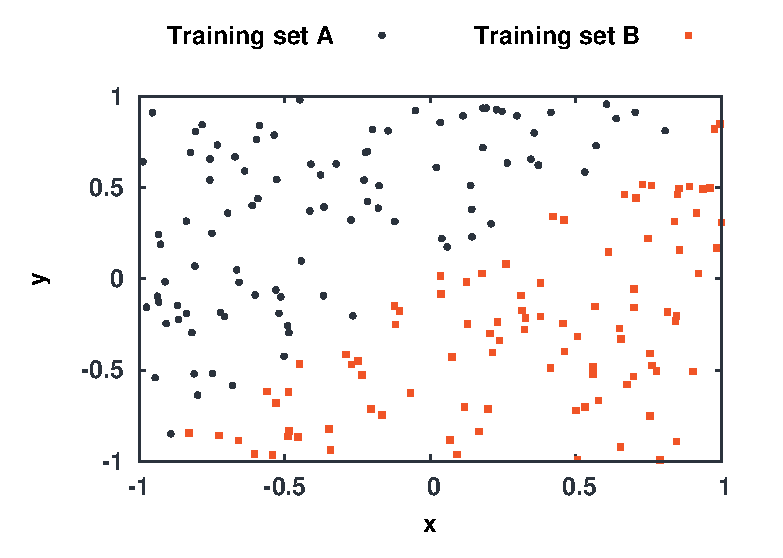
\includegraphics[width=0.48\textwidth]{figures/knn_95_85_separable_default_weighted_samples.eps} \label{fig: knnSepTrainSetDef}}
\hfill
\subfigure[Distant]{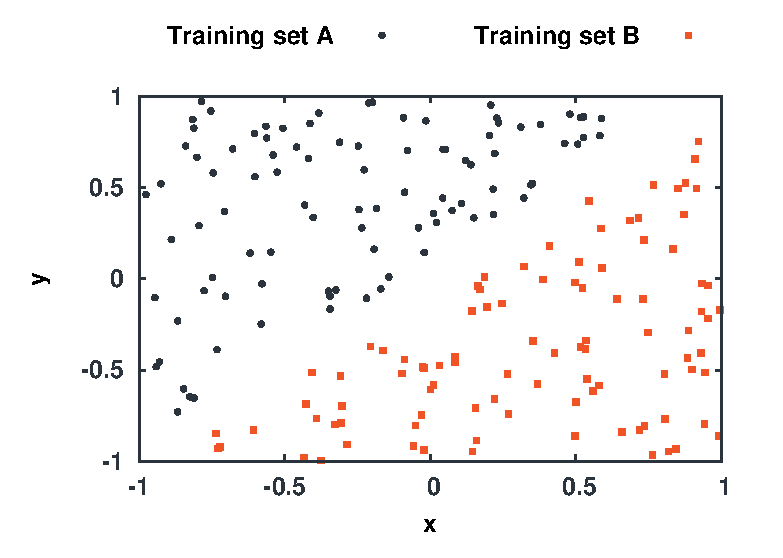
\includegraphics[width=0.48\textwidth]{figures/knn_95_85_separable_distant_weighted_samples.eps} \label{fig: knnSepTrainSetDis}}
\hfill
\centering\subfigure[Overlapped]{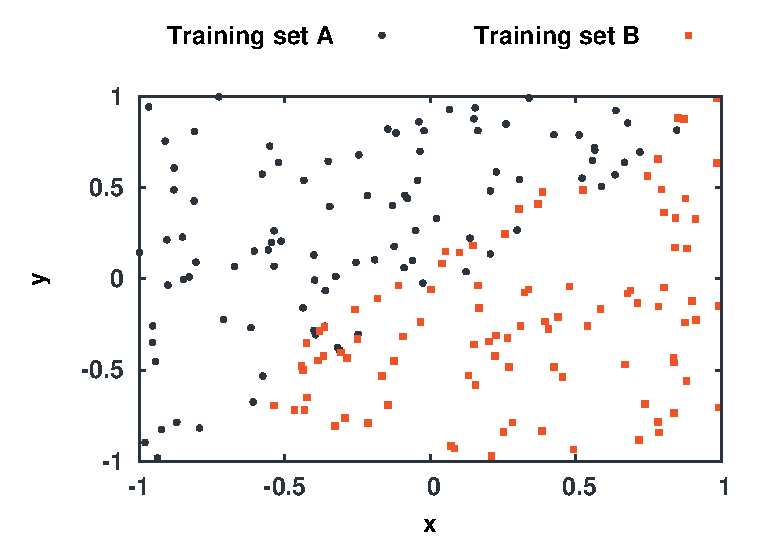
\includegraphics[width=0.48\textwidth]{figures/knn_95_55_separable_overlapped_weighted_samples.eps} \label{fig: knnSepTrainSetOvr}}
\hfill
\caption{Training sets for points separable by $f(x) = x$.}
\label{fig: knnSepTrainSet}
\end{figure}

Lets consider something defined mathematically better than {\it blue} and {\it orange}, i.e. two classes of points which can be separated linearly, e.g. by the line $f(x) = x$ as presented on Fig. \ref{fig: knnSepTrainSet} in three scenarios:

\begin{itemize}
 \item points are exactly separated by $f(x) = x$, Fig. \ref{fig: knnSepTrainSetDef}
 \item there is a small gap to make points more separated, Fig. \ref{fig: knnSepTrainSetDis}
 \item points overlap a little, Fig. \ref{fig: knnSepTrainSetOvr}
\end{itemize}

For each scenario the efficiency of kNN as a function of the size of training sets ($n$) and $k$ is checked in the following way:

\begin{enumerate}
 \item generate $n$ random points above $f(x) = x$ (training set A)
 \item generate $n$ random points below $f(x) = x$ (training set B)
 \item generate a random point
 \item find $k$ nearest neighbors of this point
 \item let them vote:
 \begin{itemize}
  \item with vote weight = $1$ (unweighted)
  \item with vote weight = $1/$distance (weighted)
 \end{itemize}
 \item repeat points 3-5 $N$ times to get good enough statistics ($N = 10^5$ for presented results)
 \item calculate the score = no. of correctly guessed points / no. of all test points
\end{enumerate}

The efficiency of kNN as a function of $k$ and $n$ can be found on Fig. \ref{fig: knnSepRes}. Clearly, weighted voting gives better results, especially for $k \sim n$. However, even unweighted kNN still gives score better than 90\%. The efficiency is almost the same when extra gap is generated between training sets (Figs. \ref{fig: knnSepResDisU} and \ref{fig: knnSepResDisW}), but it becomes much worse if training sets overlap (Figs. \ref{fig: knnSepResOvrU} and \ref{fig: knnSepResOvrW}).

\begin{figure}
\hfill
\subfigure[Default, unweighted]{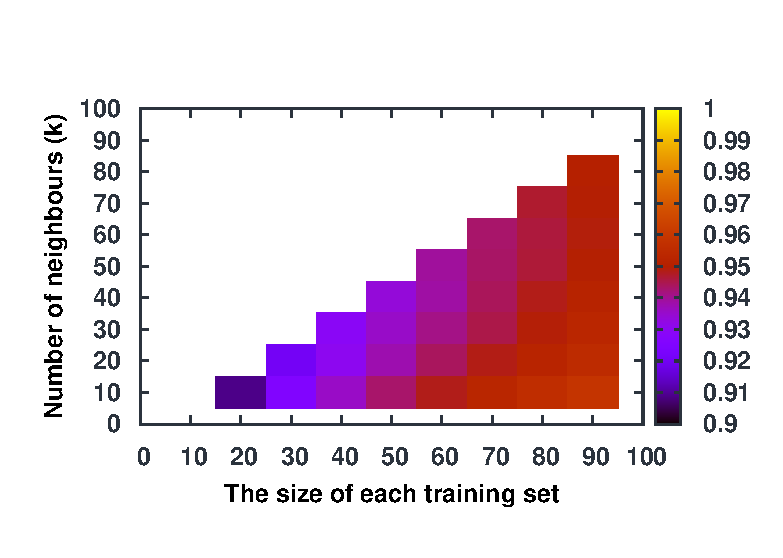
\includegraphics[width=0.48\textwidth]{figures/knn_separable_default_unweighted.eps} \label{fig: knnSepResDefU}}
\hfill
\subfigure[Default, weighted]{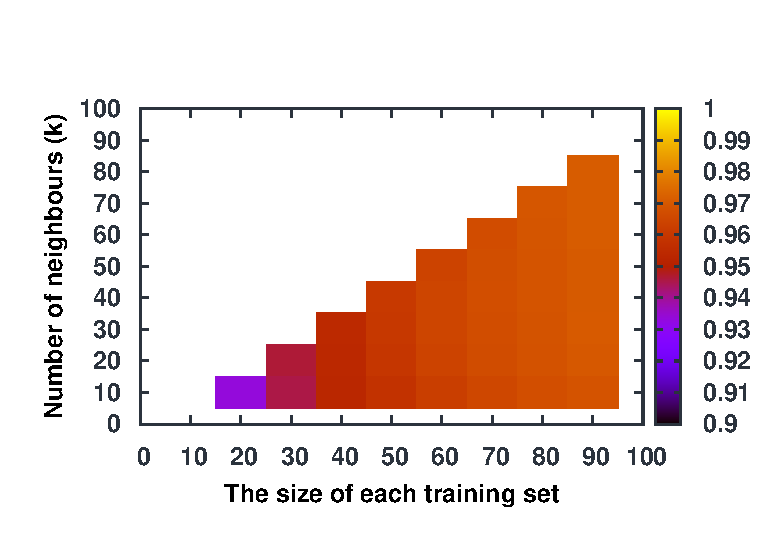
\includegraphics[width=0.48\textwidth]{figures/knn_separable_default_weighted.eps} \label{fig: knnSepResDefW}}
\hfill
\subfigure[Distant, unweighted]{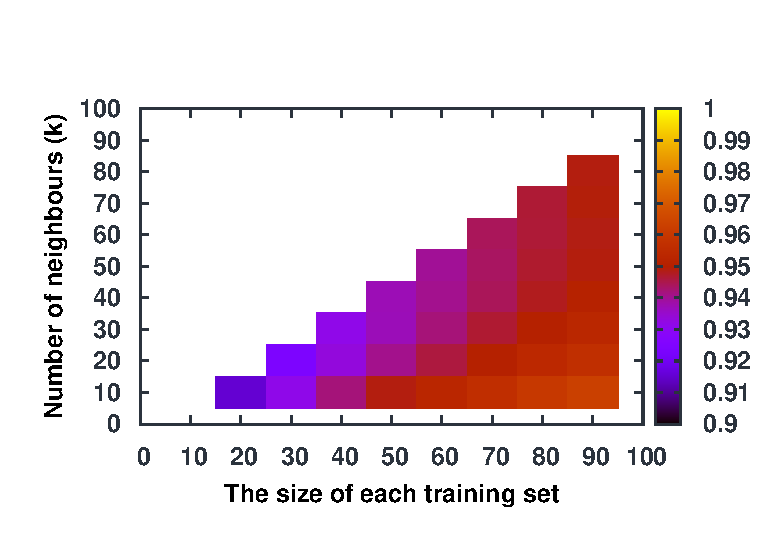
\includegraphics[width=0.48\textwidth]{figures/knn_separable_distant_unweighted.eps} \label{fig: knnSepResDisU}}
\hfill
\subfigure[Distant, weighted]{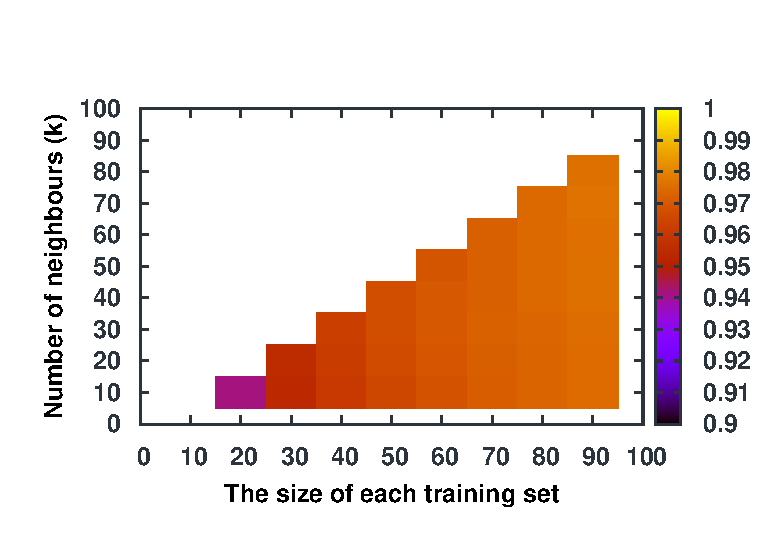
\includegraphics[width=0.48\textwidth]{figures/knn_separable_distant_weighted.eps} \label{fig: knnSepResDisW}}
\hfill
\subfigure[Overlapped, unweighted]{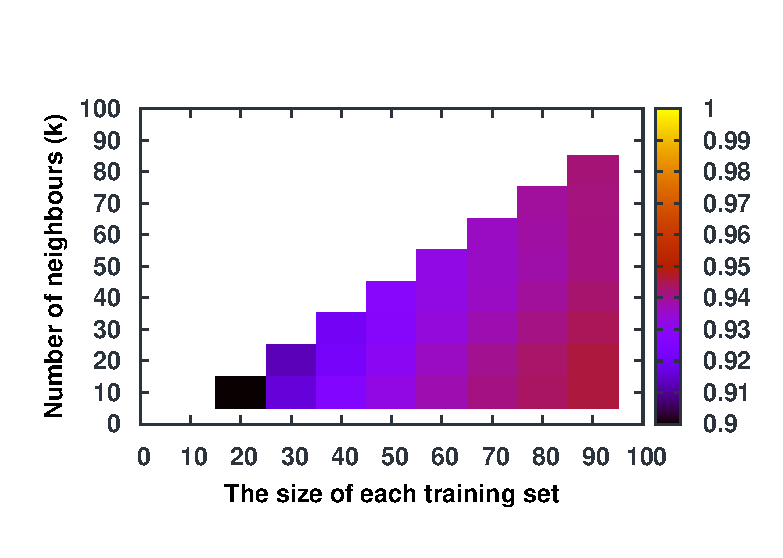
\includegraphics[width=0.48\textwidth]{figures/knn_separable_overlapped_unweighted.eps} \label{fig: knnSepResOvrU}}
\hfill
\subfigure[Overlapped, weighted]{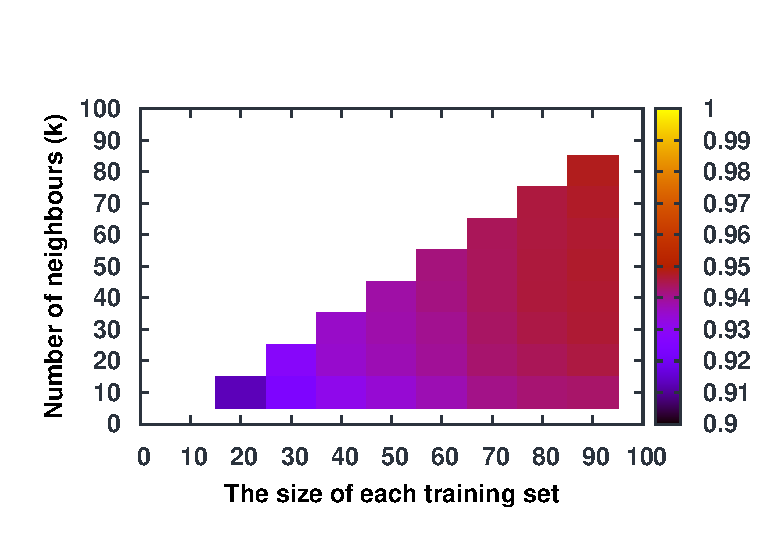
\includegraphics[width=0.48\textwidth]{figures/knn_separable_overlapped_weighted.eps} \label{fig: knnSepResOvrW}}
\hfill
\caption{kNN efficiency for points separable by $f(x) = x$.}
\label{fig: knnSepRes}
\end{figure}

\begin{figure}
\hfill
\subfigure[Training sets]{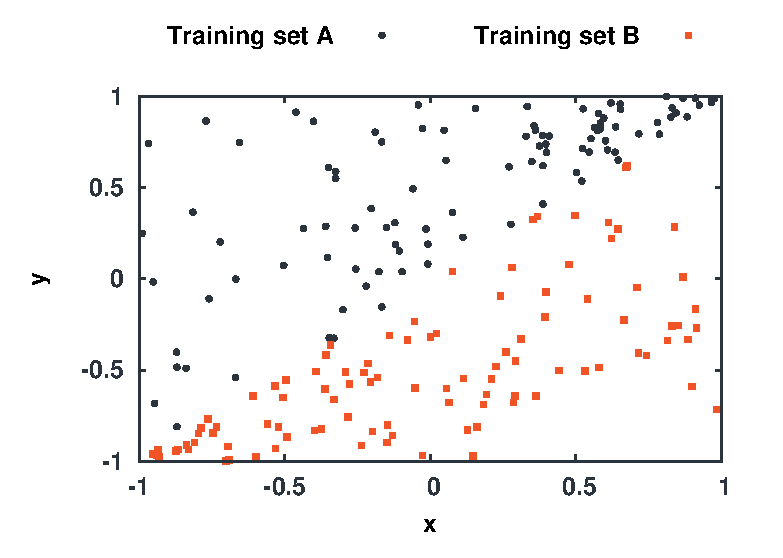
\includegraphics[width=0.48\textwidth]{figures/knnWrongTrainSet.eps} \label{fig: knnWrongTrainSet}}
\hfill
\subfigure[Testing set]{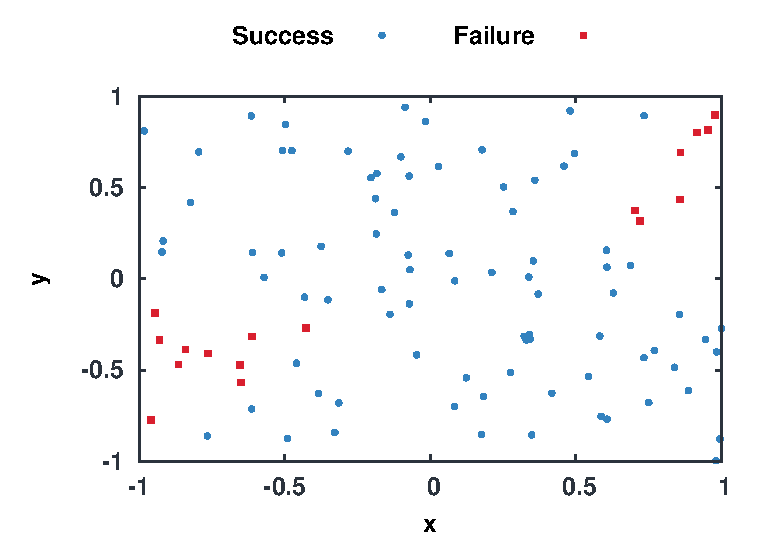
\includegraphics[width=0.48\textwidth]{figures/knnWrongTrainResults.eps} \label{fig: knnWrongTrainResults}}
\hfill
\hfill
\caption{The example of the kNN classification using wrong training sets ($n = 100$, $k = 50$).}
\label{fig: knnWrongTrain}
\end{figure}

Lets take a look what happens when training sets are not uniformly distributed, as presented on Fig. \ref{fig: knnWrongTrain}. It still looks (by eye) that training sets are separated by $f(x) = x$, see Fig. \ref{fig: knnWrongTrainSet}. However, from obvious reasons some points are going to be incorrectly classified, as presented on Fig. \ref{fig: knnWrongTrainResults}.



\section{Support Vector Machine}
\label{sec: svm}

Support Vector Machine is one those algorithms which sounds pretty easy until you actually start using it. It is a binary classifier, so it can only work with two classes at a time. It is an extension of perceptron algorithm (sometimes known as perceptron with optimal stability). 

The perceptron algorithm looks for a line (or a hyperplane in general) which separates training sets. Thus, it works only for linearly separable classes. The hyperplane is found using online learning, by updating the hyperplane based on incorrectly classified training points. For linearly separable classes it guarantees convergence, but it does not control the final orientation of the hyperplane. As presented on Fig. \ref{fig: perceptron}, there is infinitely many hyperplanes (lines) like that.

\begin{figure}
  \centering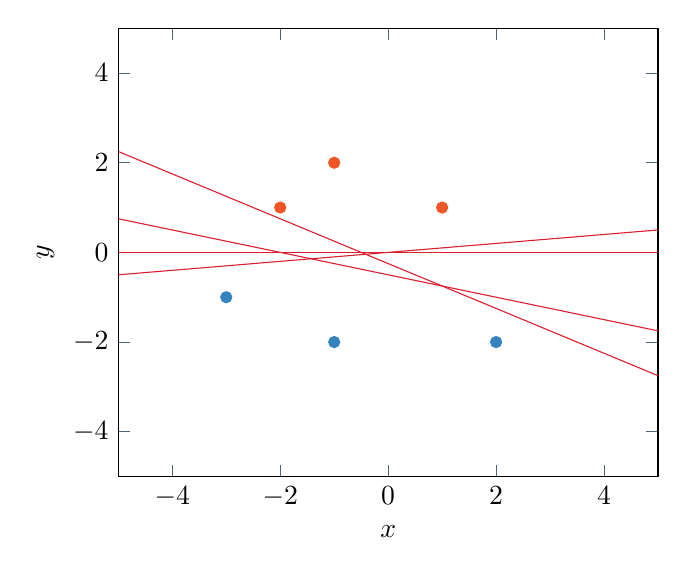
\begin{tikzpicture}

  \begin{axis}[xlabel = $x$, ylabel = $y$, xmin = -5.0, xmax = 5.0, ymin = -5.0, ymax = 5.0]
    
    \addplot[mark = *, , draw = none, color = orange] coordinates {(1,1)}; 
    \addplot[mark = *, , draw = none, color = orange] coordinates {(-1,2)}; 
    \addplot[mark = *, , draw = none, color = orange] coordinates {(-2,1)}; 

    \addplot[mark = *, , draw = none, color = blue] coordinates {(-1,-2)}; 
    \addplot[mark = *, , draw = none, color = blue] coordinates {(2,-2)}; 
    \addplot[mark = *, , draw = none, color = blue] coordinates {(-3,-1)}; 

    \addplot[color = red] {0};
    \addplot[color = red] {-0.25*x - 0.50};
    \addplot[color = red] {-0.50*x - 0.25};
    \addplot[color = red] {0.1*x};
    
    %\addplot[mark = *, , draw = none, color = red] coordinates {(-1,-1)};

  \end{axis}

\end{tikzpicture}
  \caption{Examples of separation lines for two-dimensional data.}
  \label{fig: perceptron}
\end{figure}

One can expect that the best separation hyperplane should be possible as far as possible from both testing samples. Intuitively, the ``real'' boundary separating classes (which is unknown) is located far from the center of training sets. This way, one may expect better classification of unusual testing points, so better generalization of the problem.

SVM guarantees (for linearly separable classes) finding the maximum-margin hyperplane. It can be easily extend for ``almost'' linearly separable classes, like those presented on Fig. \ref{fig: knnSepTrainSetOvr} (see Sec. \ref{sec: svmAlmost}). For classes linearly inseparable, {\it kernel trick} is used to transform feature space to higher dimension, where classes are linearly separable and maximum-margin hyperplane can be found (see Sec. \ref{sec: svmKernel}).

The task is ``easy'' - find the separation hyperplane and classification is straightforward.
\subsection{Linear SVM}
\label{fig: svmLinear}

Lets consider our training sets are given by:

\begin{equation}
  \left\{\left(\vec x_i, y_i\right)\right\}_{i=1,...,N}
  \label{eq: trainSet}
\end{equation}

where $\vec x_i = \left(x_{i1}, ... , x_{in}\right) \in \mathbb{R}^n$ are features vector in $n$-dimensional space, $y_i \in \left\{-1, 1\right\}$ defines membership to given class\footnote{$\left\{-1, 1\right\}$ was chosen for convenience in further calculations.}, $N$ is the size of training sets. A hyperplane can be defined by its normal vector ($\vec\omega = (\omega_1, ... , \omega_n)$) and an absolute term ($\omega_0$):

\begin{equation}
 \omega_0 + \underbrace{\omega_1 \cdot x_1 + ... + \omega_n\cdot x_n}_{\left<\vec\omega, \vec x\right>} = 0
 \label{eq: hyperplane}
\end{equation}

The distance ($d$) between a point $\vec x$ and a hyperplane defined by $\vec\omega$ and $\omega_0$ is given by the following formula:

\begin{equation}
 d \left(\vec x, \vec\omega, \omega_0\right) = \frac{\left|\omega_0 + \left<\vec\omega, \vec x\right>\right|}{||\vec\omega||}
 \label{eq: distance}
\end{equation}

where $||\vec\omega|| = \sqrt{\omega_1^2 + ... + \omega_n^2}$ is norm of the vector $\vec\omega$. Having that, the margin of separation ($\tau$) for training set from Eq. \ref{eq: trainSet} and a hyperplane as in Eq. \ref{eq: hyperplane} is defined as:

\begin{equation}
 \tau (\vec\omega, \omega_0) = \min_{i=1,...,N} \frac{y_i\cdot\left(\omega_0 + \left<\vec\omega, \vec x_i\right>\right)}{||\vec\omega||}
\end{equation}

so it is a distance between the hyperplane and the closest point. One should note, that absolute value from Eq. \ref{eq: distance} disappears because of smart choice of $y$ values. Points on the ``positive'' side of the hyperplane have $y = 1$, and those on the ``negative'' side have $y = -1$, which guarantees $\tau \geq 0$ (assuming all testing points are classified correctly).

\begin{figure}
 \centering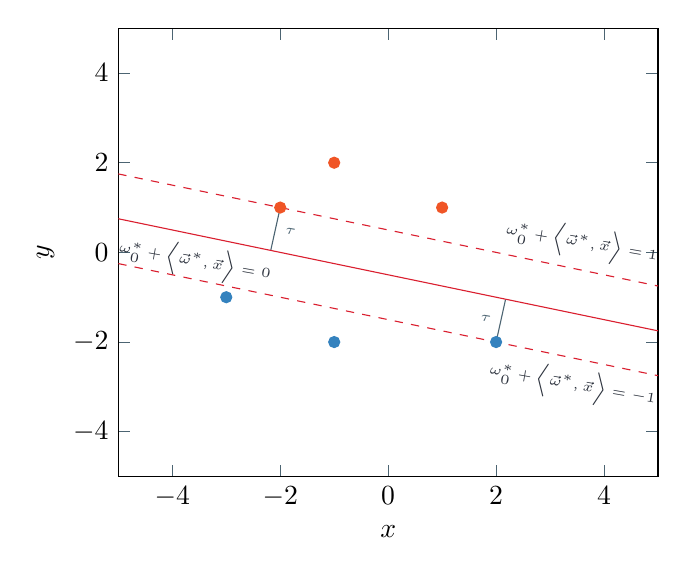
\begin{tikzpicture}

  \begin{axis}[xlabel = $x$, ylabel = $y$, xmin = -5.0, xmax = 5.0, ymin = -5.0, ymax = 5.0]
    
    \addplot[mark = *, , draw = none, color = orange] coordinates {(1,1)}; 
    \addplot[mark = *, , draw = none, color = orange] coordinates {(-1,2)}; 
    \addplot[mark = *, , draw = none, color = orange] coordinates {(-2,1)}; 

    \addplot[mark = *, , draw = none, color = blue] coordinates {(-1,-2)}; 
    \addplot[mark = *, , draw = none, color = blue] coordinates {(2,-2)}; 
    \addplot[mark = *, , draw = none, color = blue] coordinates {(-3,-1)}; 

    \addplot[mark = none, color = gray] coordinates {(-2,1) (-2.175,0.05)} node[right, pos=0.5, rotate=-10] {\tiny$\tau$}; 
    \addplot[mark = none, color = gray] coordinates {(2,-2) (2.175,-1.05)} node[left, pos=0.5, rotate=-10] {\tiny$\tau$}; 

    \addplot[color = red]         {-0.25*x - 0.5} node[below, pos=0.15, rotate=-10] {\color{black}\tiny$\omega_0^* + \left<\vec\omega^*, \vec x\right> = 0$};;
    \addplot[color = red, dashed] {-0.25*x - 1.5} node[below, pos=0.85, rotate=-10] {\color{black}\tiny$\omega_0^* + \left<\vec\omega^*, \vec x\right> = -1$};
    \addplot[color = red, dashed] {-0.25*x + 0.5} node[above, pos=0.85, rotate=-10] {\color{black}\tiny$\omega_0^* + \left<\vec\omega^*, \vec x\right> = 1$};;
    
  \end{axis}

\end{tikzpicture}
 \caption{The example of maximum-margin hyperplane separating two training sets. {\it Note, it is just a demonstrative cartoon, not real calculations.}}
 \label{fig: svmMargin}
\end{figure}

SVM is looking for the optimal hyperplane, so the one with the maximum margin of separation. The optimization task to solve is:

\begin{subequations}
 \begin{equation}
  \text{maximize}\hspace{10pt}\tau (\vec\omega, \omega_0)
 \end{equation}
 \begin{equation}
  \text{subject to}\hspace{10pt}\forall_i\hspace{5pt} y_i \cdot \left(\omega_0 + \left<\vec\omega, \vec x_i\right>\right) \geq \tau(\vec\omega, \omega_0)\cdot ||\vec\omega||
  \label{eq: optimization0C}
 \end{equation}
 \label{eq: optimization0}
\end{subequations}

Thus, maximize $\tau$ and make sure all points are on the right side of the hyperplane (with the distance not smaller than $\tau$). Please note, that there are still infinitively many hyperplanes fulfill these conditions (as multiplying Eq. \ref{eq: hyperplane} by a constant does not change the position of the hyperplane). One can use an arbitrary bond to determine the hyperplane unambiguously. It is convenient to use the following bond:

\begin{equation}
 \tau(\vec\omega, \omega_0)\cdot ||\vec\omega|| = 1
\end{equation}

With this bond, maximizing $\tau$ can be considered as minimizing the length of normal vector $||\vec\omega||$, so the optimization conditions from Eq. \ref{eq: optimization0} can be rewritten as:

\begin{subequations}
 \begin{equation}
  \text{minimize}\hspace{10pt} Q(\vec\omega) = \frac{1}{2}||\vec\omega||^2
  \label{eq: maximize}
 \end{equation}
 \begin{equation}
  \text{subject to}\hspace{10pt}\forall_i\hspace{5pt} y_i \cdot \left(\omega_0 + \left<\vec\omega, \vec x_i\right>\right) \geq 1
  \label{eq: condition}
 \end{equation}
 \label{eq: optimization}
\end{subequations}

where $\frac{1}{2}$ in Eq. \ref{eq: maximize} is just for convenience in further calculations. For the same reasons, the square of $||\vec\omega||$ is considered. It does not affect the final result as $||\vec\omega||$ and $Q(\vec\omega)$ have the minimum for the same $\vec\omega$. 

The example of maximum-margin hyperplane separating two training sets is presented on Fig. \ref{fig: svmMargin}, where $\omega_0^*$ and $\vec\omega^*$ denote the solution of Eq. \ref{eq: optimization}. Please note, this is just a demonstrative cartoon, not a real solution.

Eq. \ref{eq: optimization} is a quadratic programming problem. It is a kind of mathematical optimization which is extensively studied. There are many methods to solve this kind of problems. In the context of SVM Lagrange multipliers is commonly used. Sec. \ref{sec: lm} is an introduction / reminder on Lagrange multipliers. In Sec. \ref{sec: svmLinearLM} Eq. \ref{eq: optimization} is solved using this method.
\subsection{Lagrange multipliers}
\label{sec: lm}

Lagrange multipliers is the method to optimize (find minimum or maximum) of the function $f (\vec x) : \mathbb{R}^n \rightarrow \mathbb{R}$ with given constraint\footnote{The constraint could be given by $g (\vec x) = c$, but one can introduce $g'(\vec x) = g (\vec x) - c = 0$.} $g (\vec x) = 0$. The method is based on the fact that the gradient of the function $f$ must be parallel to the gradient of the constraint $g$:

\begin{equation}
 \nabla f (\vec x) = \lambda \nabla g (\vec x)
 \label{eq: lmBase}
\end{equation}

where $\lambda$ is a Lagrange multiplier. Why Eq. \ref{eq: lmBase} is true? Lets consider intuitive geometric explanation. If you want a strict proof grab a math book!

In general, the gradient $\nabla f$ gives the directions to head to optimize $f$. If going exactly in the direction of the gradient is impossible, but it is possible to go in the direction of a component of the gradient it still good (just increase / decrease is slower). If the gradient is perpendicular, there is no such component and the local optimum is found. Fig. \ref{fig: lmf} illustrates this.

\begin{figure}
\hfill
\subfigure[Looking of the local optimum of the function $f$.]{\scalebox{0.8}{\begin{tikzpicture}

  \begin{axis}[axis lines = none, axis equal]
    

    \addplot[mark = none, color = morange, thick, ->, >=latex] coordinates {(0.0, 1.0) (0.0, 1.25)};

    \addplot[mark = none, color = morange, thick, ->, >=latex] coordinates {(-0.5, 0.75) (-0.5, 1.0)};
    
    \addplot[smooth, color = mblack, thick, domain = -0.6:0.6] {-x*x + 1} node[above, pos = 0.75] {\color{mgray}$f$};
    
    \addplot[color = mgray, thick, dashed, domain = -0.35:-0.65] {x + 1.25};
    \addplot[color = mgray, thick, dashed, domain = -0.35:-0.65] {-x + 0.25};
    
    \addplot[mark = none, color = mblue, thick, ->, >=latex] coordinates {(-0.5, 0.75) (-0.4, 0.85)};

    \node(grad) [color = mgray] at (axis cs:-0.3,1.25) {\tiny gradients};
    
    \draw [color = mgray, ->, >=latex, shorten >= 2pt] (grad) -- (axis cs:0.0, 1.1);
    \draw [color = mgray, ->, >=latex, shorten >= 2pt] (grad) -- (axis cs:-0.5, 1.0);
    
    \node(move) [color = mgray] at (axis cs: 0.0, 0.75) {\tiny the direction of movement};
    
    \draw [color = mgray, ->, >=latex, shorten >= 2pt] (move.west) -- (axis cs:-0.45, 0.8);
    
    \node(nomove) [color = mgray, text width = 10cm, align = center] at (axis cs: 0.4, 1.2) {\tiny perpendicular gradient \\ no more moves \\};
    
    \draw [color = mgray, ->, >=latex, shorten >= 2pt] (nomove) -- (axis cs:0.0, 1.0);
    
  \end{axis}

\end{tikzpicture}} \label{fig: lmf}}
\hfill
\subfigure[Moving along the constraint $g$.]{\scalebox{0.8}{\begin{tikzpicture}

  \begin{axis}[axis lines = none, axis equal]
            
    \addplot[mark = none, color = mgreen, thick, ->, >=latex] coordinates {(-0.7, -0.343) (-0.9, -0.207)};
    
    \addplot[mark = none, color = morange, thick, ->, >=latex] coordinates {(-0.7, -0.343) (-0.8, 0.0)};

    \addplot[mark = none, color = morange, thick, ->, >=latex] coordinates {(0.5, 0.125) (0.3, 0.391)};    

    \addplot[mark = none, color = mgreen, thick, ->, >=latex] coordinates {(0.5, 0.125) (0.4, 0.258)};    
    
    \addplot[smooth, color = mblack, thick, domain = -1:1] {x*x*x} node[right, pos = 0.75] {\color{mgray}$g$};
    
    \addplot[mark = none, color = mblue, thick, ->, >=latex] coordinates {(-0.7, -0.343) (-0.6, -0.2)};
    
    \node(grad) [color = mgray] at (axis cs:-0.5,0.5) {\tiny gradients of $f$};

    \draw [color = mgray, ->, >=latex, shorten >= 2pt] (grad) -- (axis cs:-0.8,0);
    \draw [color = mgray, ->, >=latex, shorten >= 2pt] (grad) -- (axis cs:0.3, 0.391);
    
    \node(gradg) [color = mgray, text width = 3cm, align = center] at (axis cs:-0.3,-0.8) {\tiny gradients of $g$ \\ always perpendicular to $g$ \\};
    
    \draw [color = mgray, ->, >=latex, shorten >= 2pt] ([xshift=-1cm] gradg.north) -- (axis cs:-0.8, -0.3);
    
    \node(dir) [color = mgray, text width = 5cm, align = left] at (axis cs:0.4,-0.5) {\tiny the direction of movement \\ must be perpendicular to $\nabla g$ \\};
    
    \draw [color = mgray, ->, >=latex, shorten >= 2pt] (dir) -- (axis cs:-0.65,-0.3);
    
    \node(end) [color = mgray, text width = 3cm, align = center] at (axis cs:0.6,-0.2) {\tiny $\nabla f \parallel \nabla g$ \\ no more moves\\};
    
    \draw [color = mgray, ->, >=latex, shorten >= 2pt] (end) -- (axis cs:0.5,0.125);
    
  \end{axis}

\end{tikzpicture}} \label{fig: lmg}}
\hfill
\caption{The illustration of constraint optimization.}
\end{figure}

If constraint $g = 0$ is given, the movement is restricted to fulfill the condition. In other words, only moves along $g$ are possible. To keep $g$ constant, only moves perpendicular to the gradient of $g$ are allowed (otherwise increase or decrease of $g$ would occur). This is demonstrated on Fig. \ref{fig: lmg}. The direction of the movement is determined by $\nabla g$ (must be perpendicular) and $\nabla f$. More precisely it is given by a component of $\nabla f$ perpendicular to $\nabla g$. If $\nabla f$ is parallel to $\nabla g$ there is no such component and the local optimum (fulfilling the constraint) is found.

For convenience, lets introduce Lagrangian defined as:

\begin{equation}
 \mathcal{L} (\vec x, \lambda) = f (\vec x) - \lambda g (\vec x)
 \label{eq: lagrangian0}
\end{equation}

so the Eq. \ref{eq: lmBase} can be rewritten as:

\begin{equation}
 \nabla \mathcal{L} (\vec x, \lambda) = 0
 \label{eq: lagrEq}
\end{equation}

Lets go back to SVM optimization problem defined by Eq. \ref{eq: optimization}. The number of constraints there is equal to the size of the training set ($N$). Fortunately, the generalization of the Lagrangian (Eq. \ref{eq: lagrangian0}) is straightforward:

\begin{equation}
 \mathcal{L} (\vec x, \lambda_1, ..., \lambda_N) = f (\vec x) - \sum_{i = 1}^N\lambda_i g_i (\vec x)
 \label{eq: lagrangian}
\end{equation}

where $\lambda_i$ is Lagrange multiplier for the constraint $g_i$. The reasoning stays the same, but the movement of $f$ is now restricted by many constrains:

\begin{eqnarray*}
 \nabla f (\vec x) & = &  \lambda_1 \nabla g_1 (\vec x) \\
 \nabla f (\vec x) & = &  \lambda_2 \nabla g_2 (\vec x) \\
			 & ... & \\
 \nabla f (\vec x) & = &  \lambda_N \nabla g_N (\vec x)
\end{eqnarray*}

There is still one piece missing. The optimization problem given by Eq. \ref{eq: optimization} is constrained by inequalities. The generalization of Lagrange multipliers method to inequality constrains is given by Karush–Kuhn–Tucker (KKT) conditions, described in Sec. \ref{sec: kkt}.


\subsection{Karush–Kuhn–Tucker conditions}
\label{sec: kkt}
\subsection{Linear SVM using Lagrange multipliers}
\label{sec: svmLinearLM}

Lets go back to SVM optimization problem defined by Eq. \ref{eq: optimization} and introduce the Lagrangian $\mathcal{L} (\vec x, \lambda_1, ..., \lambda_N) \equiv \mathcal{L} (\vec x, \lambda, \mu$ defined by:

\begin{equation} 
  \mathcal{L} (\vec x, \lambda, \mu) = \frac{1}{2}||\vec\omega||^2 - \sum_{i=1}^N \lambda_i \cdot \left(y_i \cdot \left(\omega_0 + \left<\vec\omega, \vec x_i\right>\right) - 1\right)
  \label{eq: svmL}
\end{equation}

where $\lambda_i \geq 0$ as discussed in Sec. \ref{sec: kkt}. Note, that having $\lambda_i = \infty$ gives the trivial minimum at $-\infty$. In fact, one needs to minimize $\mathcal{L}$ respect to $||\omega||$ and maximize respect to $\lambda_i$. The solution is given by a saddle point, as demonstrated on Fig. \ref{fig: spoint}.

\begin{figure}
 \centering\pgfplotsset{
colormap={mycolors}{color(0cm)=(white); color(1cm)=(mgreen!75!mblue)}
}

\pgfplotsset{ticks=none}

\begin{tikzpicture}

\begin{axis}[
  colormap name=mycolors,
  view={30}{30},
  domain=-100:100,
  xlabel=$||\vec\omega||$,
  ylabel=$\lambda_i$,
  zlabel=$\mathcal{L}$,
  zlabel style={rotate=-90}
]

\addplot3 [surf] {x^2 - y^2};
\addplot3 [mark = *, , draw = none, color = mred] coordinates {(0.0, 0.0, 0.0)} node[pin=80:{\color{mred}\small saddle point}]{};

\end{axis}
\end{tikzpicture}
 \caption{The cartoon demonstrating the saddle point.}
 \label{fig: spoint}
\end{figure}

The necessity condition for a saddle point requires all partial derivatives to be zero:

\begin{subequations}
 \begin{equation}
  \frac{\partial\mathcal{L}}{\partial\vec\omega} = 0
  \label{eq: spoint1}
 \end{equation}
 \begin{equation}
  \frac{\partial\mathcal{L}}{\partial\omega_0} = 0
  \label{eq: spoint2}
 \end{equation}
 \begin{equation}
  \forall_i \hspace{10pt} \frac{\partial\mathcal{L}}{\partial\lambda_i} = 0
  \label{eq: spoint3}
 \end{equation}
 \label{eq: spoint}
\end{subequations}

From Eq. \ref{eq: spoint1}:

\begin{equation}
 \vec\omega = \sum_{i=1}^N \lambda_iy_i\vec x_i
 \label{eq: from1}
\end{equation}

and from Eq. \ref{eq: spoint2}:

\begin{equation}
 \sum_{i=1}^{N} \lambda_iy_i = 0
 \label{eq: from2}
\end{equation}

Lets use Eqs. \ref{eq: svmL}, \ref{eq: from1} and \ref{eq: from2} to express the Lagrangian only in terms of $\lambda_i$:

\begin{eqnarray}
  \mathcal{L} (\vec x, \lambda, \mu) & = & \frac{1}{2}||\vec\omega||^2 - \sum_{i=1}^N \lambda_i \cdot \left(y_i \cdot \left(\omega_0 + \left<\vec\omega, \vec x_i\right>\right) - 1\right) \\ \nonumber
  & = & \frac{1}{2}\left<\vec\omega, \vec\omega\right> - \omega_0 \sum_{i=1}^N \lambda_iy_i - \sum_{i=1}^N\lambda_iy_i\left<\vec\omega, \vec x_i\right> + \sum_{i=1}^{N}\lambda_i \\ \nonumber
  & = & \frac{1}{2}\sum_{i=1}^N\sum_{j=1}^N\lambda_i\lambda_jy_iy_j\left<\vec x_i, \vec x_j\right> - 0 - \sum_{i=1}^N\sum_{j=1}^N\lambda_i\lambda_jy_iy_j\left<\vec x_i, \vec x_j\right> + \sum_{i=1}^{N}\lambda_i \\ \nonumber
  & = & -\frac{1}{2}\sum_{i=1}^N\sum_{j=1}^N\lambda_i\lambda_jy_iy_j\left<\vec x_i, \vec x_j\right> + \sum_{i=1}^{N}\lambda_i
\end{eqnarray}

Finally, only the maximization of $\mathcal{L}$ respect to $\lambda_i$ must be performed, so the problem now is defined as:

\begin{eqnarray}
 \text{maximize} & & \mathcal{L} (\vec x, \lambda, \mu) = -\frac{1}{2}\sum_{i=1}^N\sum_{j=1}^N\lambda_i\lambda_jy_iy_j\left<\vec x_i, \vec x_j\right> + \sum_{i=1}^{N}\lambda_i \\ \nonumber
 \text{subject to} & & \forall_i \hspace{10pt} \lambda_i \geq 0 \\ \nonumber
 \text{} & & \sum_{i=1}^{N} \lambda_iy_i = 0
 \label{eq: optimizationLM}
\end{eqnarray}

Usually, most of $\lambda_i$ are equal zero. Vectors $\vec x_i$ which correspond to $\lambda_i > 0$ are called support vectors (and suddenly the name of the method is clear!). According to Eq. \ref{eq: from1}, the normal vector $\vec\omega$ is linear combinations of support vectors. Take a look at Fig. \ref{fig: svmMargin}. Support vectors are those lying on $\omega_0^* + \left<\vec\omega^*, \vec x\right> = \pm 1$. The last piece is the absolute term $\omega_0$, which can be calculated from any constraint (for any support vector):

\begin{eqnarray}
 y_i \cdot \left(\omega_0 + \left<\vec\omega, \vec x_i\right>\right) - 1 & = & 0 \\ \nonumber
 y_i\omega_0 & = & 1 - y_i \left<\vec\omega, \vec x_i\right> \\ \nonumber
 \omega_0 & = & y_i - \left<\vec\omega, \vec x_i\right>
\end{eqnarray}


\subsection{Soft margin}
\label{sec: svmLinearSoft}

So far, only perfectly separable cases were discussed, with the hyperplane which exactly separates two training sets (like presented on Figs. \ref{fig: knnSepTrainSetDef} and \ref{fig: knnSepTrainSetDis}). It is so called SVM with hard margin. It is clearly going to fail if training sets overlapped (like presented on Fig. \ref{fig: knnSepTrainSetOvr}). There is a simple extension to SVM method which allows some points to exists within the margin (between $\omega_0^* + \left<\vec\omega^*, \vec x\right> = 0$ and $\omega_0^* + \left<\vec\omega^*, \vec x\right> = \pm 1$ on Fig. \ref{fig: svmMargin}). It is so called SVM with soft margin. 

\begin{figure}
 \centering\begin{tikzpicture}

  \begin{axis}[xlabel = $x$, ylabel = $y$, xmin = -5.0, xmax = 5.0, ymin = -5.0, ymax = 5.0]
    
    \addplot[mark = *, , draw = none, color = morange] coordinates {(1,1)}; 
    \addplot[mark = *, , draw = none, color = morange] coordinates {(-1,2)}; 
    \addplot[mark = *, , draw = none, color = morange] coordinates {(-2,1)}; 

    \addplot[mark = *, , draw = none, color = mblue] coordinates {(-1,-2)}; 
    \addplot[mark = *, , draw = none, color = mblue] coordinates {(2,-2)}; 
    \addplot[mark = *, , draw = none, color = mblue] coordinates {(-3,-1)}; 

    \addplot[mark = *, , draw = none, color = mblue] coordinates {(0,-0.8)}; 
    \addplot[mark = none, color = mgray] coordinates {(0,-0.8) (-0.12, -1.45)} node[right, pos=0.5, rotate=-10] {\tiny$\varepsilon < \tau$}; 

    \addplot[mark = *, , draw = none, color = morange] coordinates {(-1,-0.5)}; 
    \addplot[mark = none, color = mgray] coordinates {(-1,-0.5) (-0.75, 0.7)} node[right, pos=0.5, rotate=-10] {\tiny$\varepsilon > \tau$}; 

    
    \addplot[mark = none, color = mgray] coordinates {(-2,1) (-2.175,0.05)} node[right, pos=0.5, rotate=-10] {\tiny$\tau$}; 
    \addplot[mark = none, color = mgray] coordinates {(2,-2) (2.175,-1.05)} node[left, pos=0.5, rotate=-10] {\tiny$\tau$}; 

    \addplot[color = mred]         {-0.25*x - 0.5} node[below, pos=0.15, rotate=-10] {\color{mblack}\tiny$\omega_0^* + \left<\vec\omega^*, \vec x\right> = 0$};;
    \addplot[color = mred, dashed] {-0.25*x - 1.5} node[below, pos=0.85, rotate=-10] {\color{mblack}\tiny$\omega_0^* + \left<\vec\omega^*, \vec x\right> = -1$};
    \addplot[color = mred, dashed] {-0.25*x + 0.5} node[above, pos=0.85, rotate=-10] {\color{mblack}\tiny$\omega_0^* + \left<\vec\omega^*, \vec x\right> = 1$};;
    
    
  \end{axis}

\end{tikzpicture}
 \caption{The example of soft margin. {\it Note, it is just a demonstrative cartoon, not real calculations.}}
 \label{fig: svmSoftMargin}
\end{figure}

Lets associate the error $\varepsilon_i$ with every feature vector $\vec x_i$. The error defines how deep into the margin $\vec x_i$ falls:

\begin{itemize}
 \item[$\varepsilon_i = 0$] $\vec x_i$ is outside the margin
 \item[$\tau > \varepsilon_i > 0$] $\vec x_i$ is inside the margin but on the right side of the hyperplane
 \item[$\varepsilon_i > \tau$] $\vec x_i$ is on the wrong side of the hyperplane
\end{itemize}

as presented on Fig. \ref{fig: svmSoftMargin}. It requires to modify constraints defined by Eq. \ref{eq: optimization0C}:

\begin{equation}
  \forall_i\hspace{5pt} y_i \cdot \left(\omega_0 + \left<\vec\omega, \vec x_i\right>\right) + \varepsilon_i||\vec\omega||\geq \tau(\vec\omega, \omega_0)\cdot ||\vec\omega|| 
\end{equation}

After applying normalization bond $||\tau\cdot\vec\omega|| = 1$ the new constraints may be written as:

\begin{equation}
  \forall_i\hspace{5pt} y_i \cdot \left(\omega_0 + \left<\vec\omega, \vec x_i\right>\right) + \xi_i\geq 1
  \label{eq: softCsr}
\end{equation}

where $\xi_i \equiv \varepsilon_i||\vec\omega||$ is introduced for convenience. Once again the goal is to maximize $\tau$, so minimize $||\vec\omega||$, but also to minimize the errors $\xi_i$, with constraints defined by Eq. \ref{eq: softCsr}. In other words:

\begin{eqnarray}
 \text{minimize} & & Q(\vec\omega, \xi_1, ... , \xi_N) = \frac{1}{2}||\vec\omega||^2 + C\sum_{i=1}^N\xi_i \\ \nonumber
 \text{subject to} & & \forall_i\hspace{5pt} y_i \cdot \left(\omega_0 + \left<\vec\omega, \vec x_i\right>\right) + \xi_i\geq 1 \\ \nonumber
 \text{} & & \xi_i \geq 0
 \label{eq: optimizationSoft}
\end{eqnarray}

where $C > 0$ is a free parameter. Small $C$ makes the second term of $Q$ less important. It means the optimization is focused on finding large $\tau$ even for a price of having large errors $\xi_i$. On the other hand, large $C$ makes the optimization more sensitive to errors $\xi_i$ so small margin $\tau$ is preferred to minimize errors. It is demonstrated on Fig. \ref{fig: svmSoftMarginC}.

\begin{figure}
\hfill
\subfigure[Large $C$]{\begin{tikzpicture}[scale=0.7]

  \begin{axis}[xlabel = $x$, ylabel = $y$, xmin = -5.0, xmax = 5.0, ymin = -5.0, ymax = 5.0]
    
    \addplot[mark = *, , draw = none, color = morange] coordinates {(1,1)}; 
    \addplot[mark = *, , draw = none, color = morange] coordinates {(-1,2)}; 
    \addplot[mark = *, , draw = none, color = morange] coordinates {(-2,1)}; 

    \addplot[mark = *, , draw = none, color = mblue] coordinates {(-1,-2)}; 
    \addplot[mark = *, , draw = none, color = mblue] coordinates {(2,-2)}; 
    \addplot[mark = *, , draw = none, color = mblue] coordinates {(-3,-1)}; 

    \addplot[mark = *, , draw = none, color = mblue] coordinates {(0,-0.8)}; 

    \addplot[mark = *, , draw = none, color = morange] coordinates {(-1,-0.5)}; 
    
    \addplot[color = mred]         {-0.25*x - 0.5};
    \addplot[color = mred, dashed] {-0.25*x - 1};
    \addplot[color = mred, dashed] {-0.25*x + 0};   
    
  \end{axis}

\end{tikzpicture}}
\hfill
\subfigure[Small $C$]{\begin{tikzpicture}[scale=0.7]

  \begin{axis}[xlabel = $x$, ylabel = $y$, xmin = -5.0, xmax = 5.0, ymin = -5.0, ymax = 5.0]
    
    \addplot[mark = *, , draw = none, color = morange] coordinates {(1,1)}; 
    \addplot[mark = *, , draw = none, color = morange] coordinates {(-1,2)}; 
    \addplot[mark = *, , draw = none, color = morange] coordinates {(-2,1)}; 

    \addplot[mark = *, , draw = none, color = mblue] coordinates {(-1,-2)}; 
    \addplot[mark = *, , draw = none, color = mblue] coordinates {(2,-2)}; 
    \addplot[mark = *, , draw = none, color = mblue] coordinates {(-3,-1)}; 

    \addplot[mark = *, , draw = none, color = mblue] coordinates {(0,-0.8)}; 

    \addplot[mark = *, , draw = none, color = morange] coordinates {(-1,-0.5)}; 
    
    \addplot[color = mred]         {-0.25*x - 0.5};
    \addplot[color = mred, dashed] {-0.25*x - 2};
    \addplot[color = mred, dashed] {-0.25*x + 1};   
    
  \end{axis}

\end{tikzpicture}}
\hfill
\caption{The example of different choices of parameter $C$. {\it Note, it is just a demonstrative cartoon, not real calculations.}}
\label{fig: svmSoftMarginC}
\end{figure}


\subsection{Linear SVM with soft margin using Lagrange multipliers}
\label{sec: svmLinearSoftLM}

For the soft margin the procedure is the same as explained in Sec. \ref{sec: svmLinearLM}, but now the optimization requires also minimization of errors with the constraint $\xi_i \geq 0$. Lets define the Lagrangian as:

\begin{equation} 
  \mathcal{L} (\vec x, \lambda, \mu) = \frac{1}{2}||\vec\omega||^2 + C\sum_{i=1}^N\xi_i - \sum_{i=1}^N \lambda_i \cdot \left(y_i \cdot \left(\omega_0 + \left<\vec\omega, \vec x_i\right>\right) - 1 + \xi_i\right) - \sum_{i=1}^N\mu_i\xi_i
  \label{eq: svmSoftL}
\end{equation}

The necessity condition for a saddle point stays the same as in Eq. \ref{eq: spoint} and the new one appears:

\begin{equation}
 \forall_i \hspace{10pt} \frac{\partial\mathcal{L}}{\partial\xi_i} = 0 \Rightarrow \lambda_i = C - \mu_i
\end{equation}

which makes $C$ an upper boundary for $\lambda_i$, so now $0 \leq \lambda_i \leq C$. Calculations like in Sec. \ref{sec: svmLinearLM} can be done to make $\mathcal{L}$ depend only on $\lambda_i$:

\begin{eqnarray}
  \mathcal{L} (\vec x, \lambda, \mu) & = & \frac{1}{2}||\vec\omega||^2 + C\sum_{i=1}^N\xi_i - \sum_{i=1}^N \lambda_i \cdot \left(y_i \cdot \left(\omega_0 + \left<\vec\omega, \vec x_i\right>\right) - 1 + \xi_i\right) - \sum_{i=1}^N\mu_i\xi_i \nonumber \\
  & = & -\frac{1}{2}\sum_{i=1}^N\sum_{j=1}^N\lambda_i\lambda_jy_iy_j\left<\vec x_i, \vec x_j\right> - \sum_{i=1}^{N}\lambda_i (\xi_i - 1) + \sum_{i=1}^NC\xi_i - \sum_{i=1}^N\mu_i\xi_i \nonumber \\
  & = & -\frac{1}{2}\sum_{i=1}^N\sum_{j=1}^N\lambda_i\lambda_jy_iy_j\left<\vec x_i, \vec x_j\right> - \sum_{i=1}^{N}\lambda_i (\xi_i - 1) + \sum_{i=1}^N(\lambda_i + \mu_i)\xi_i - \sum_{i=1}^N\mu_i\xi_i \nonumber \\
  & = & -\frac{1}{2}\sum_{i=1}^N\sum_{j=1}^N\lambda_i\lambda_jy_iy_j\left<\vec x_i, \vec x_j\right> + \sum_{i=1}^{N}\lambda_i
\end{eqnarray}

Finally, the only difference between optimizing SVM with hard margin (see Eq. \ref{eq: optimizationLM}) and soft margin is the upper boundary on $\lambda_i$ defined by the free parameter $C$:

\begin{eqnarray}\label{eq: optimizationSoftLM}
 \text{maximize} & & \mathcal{L} (\vec x, \lambda) = -\frac{1}{2}\sum_{i=1}^N\sum_{j=1}^N\lambda_i\lambda_jy_iy_j\left<\vec x_i, \vec x_j\right> + \sum_{i=1}^{N}\lambda_i \\ \nonumber
 \text{subject to} & & \forall_i \hspace{10pt} 0 \leq \lambda_i \leq C \\ \nonumber
 \text{} & & \sum_{i=1}^{N} \lambda_iy_i = 0
\end{eqnarray}

\subsection{Sequential Minimal Optimization}
\label{sec: smo}

\subsubsection{Summary of linear SVM problem}

The hyperplane, given by:

\begin{equation}
 z = \omega_0 + \left<\vec\omega, \vec x\right>
\end{equation}

separates classes for $z = 0$. The nearest points lie on $z = \pm 1$. The normal vector can be calculated from:

\begin{equation}
 \vec\omega = \sum_{i=1}^{N} \lambda_i y_i \vec x_i
 \label{eq: smoOmega}
\end{equation}

where $N$ is the number of learning samples, $\vec x_i$ is $i$-th feature vector and $y_i$ - corresponding class membership ($\left\{-1, 1\right\}$). $\lambda_i$ are Lagrange (KKT) multipliers, which can be obtained from Eq. \ref{eq: optimizationSoftLM}. Free parameter $\omega_0$ can be calculated from (for any support vector):

\begin{equation}
 \omega_0 = y_i - \left<\vec\omega, \vec x_i\right>
 \label{eq: smoOmega0}
\end{equation}

Using Eq. \ref{eq: smoOmega}, the hyperplane equation can be rewritten in the following form:

\begin{equation}
 z (\vec x) = \sum_{i=1}^N \lambda_i y_i \left<\vec x_i, \vec x\right> + \omega_0
\end{equation}

Each training sample must fulfill the KKT conditions, in this case given by:

\begin{eqnarray}
 \lambda_i = 0 & \Leftrightarrow & y_i z_i \geq 1 \\
 0 < \lambda_i < C & \Leftrightarrow & y_i z_i = 1 \\
 \lambda_i = C & \Leftrightarrow & y_i z_i \leq 1
\end{eqnarray}

where $z_i = z (\vec x_i)$ is the output for $i$-th training sample. Lets understand why. From complementary slackness condition (Eq. \ref{eq: kktCS}):

\begin{eqnarray}
 \lambda_i (y_i z_i - 1 + \xi_i) & = & 0 \\
 \mu_i \xi_i & = & 0
\end{eqnarray}

If $\lambda_i = 0$, then $\mu_i = C$ (from Eq. \ref{eq: lambdamu}), so $\xi_i = 0$ and the constraint (Eq. \ref{eq: optimizationSoft}) becomes:

\begin{equation}
 y_i z_i - 1 + \xi_i \geq 0 \Rightarrow y_i z_i - 1 \geq 0
\end{equation}

If $\lambda_i > 0$, then $y_i z_i - 1 + \xi_i = 0$. If $0 < \lambda < C$, then $\mu_i > 0$, so $\xi_i = 0$ and $y_i z_i - 1 = 0$. If $\lambda = C$, then $\mu_i = 0$, so $\xi_i \geq 0$ and $y_i z_i - 1 \leq 0$.

\subsubsection{SMO algorithm}

Sequential Minimal Optimization (SMO) algorithm was developed by John C. Platt\footnote{{\it Sequential Minimal Optimization: A Fast Algorithm for Training Support Vector Machines}, J.C. Platt, Microsoft Research, Technical Report MSR-TR-98-14.}. The method solves the smallest possible optimization problem at a time. In this case, it means updating two Lagrange multipliers in a step. Why two? To preserve a linear equality constraint ($\sum\limits_{i=1}^N\lambda_iy_i = 0$). It guarantees convergence through Osuna's theorem\footnote{{\it An improved training algorithm for support vector machines}, E. Osuna et al., In Proc. of IEEE NNSP’97, 1997}, which states that the global training problem can be broken down into a sequence of smaller subproblems.

\mbox{}\\
\noindent\textbf{Updating two Lagrange multipliers}
\mbox{}\\

\begin{figure}
\hfill
\subfigure[$y_a \neq y_b \Rightarrow \lambda_a - \lambda_b = \gamma$]{\begin{tikzpicture}
  
  \draw[thick, color = mgray] (1, 0) -- (3, 2);
  \draw[color = mblack, fill = mblue] (1.7, 0.7) circle (0.1);
  \draw[ultra thick, color = mblack] (0, 0) -- node[below] {$\lambda_b = 0$} (3, 0) -- node[right] {$\lambda_a = C$} (3, 3) -- node[above] {$\lambda_b = C$} (0, 3) -- node[left] {$\lambda_a = 0$} (0, 0);
  
\end{tikzpicture}
 \label{fig: smoUpdateM}}
\hfill
\subfigure[$y_a = y_b \Rightarrow \lambda_a + \lambda_b = \gamma$]{\begin{tikzpicture}
    
  \draw[thick, color = mgray] (2, 0) -- (0, 2);
  \draw[color = mblack, fill = mblue] (1.3, 0.7) circle (0.1);  
  \draw[ultra thick, color = mblack] (0, 0) -- node[below] {$\lambda_b = 0$} (3, 0) -- node[right] {$\lambda_a = C$} (3, 3) -- node[above] {$\lambda_b = C$} (0, 3) -- node[left] {$\lambda_a = 0$} (0, 0);
  
\end{tikzpicture}
 \label{fig: smoUpdateP}}
\hfill
\caption{Possible relations for two Lagrange multipliers. Picture ``cloned'' from {\it Sequential Minimal Optimization: A Fast Algorithm for Training Support Vector Machines}, J.C. Platt, Microsoft Research, Technical Report MSR-TR-98-14.}
\label{fig: smoUpdate}
\end{figure}

Lets assume at least one of Lagrange multipliers ($\lambda_a$, $\lambda_b$) violates KKT conditions. Both multipliers must be updated to preserve $\gamma = y_a\lambda_a + y_b\lambda_b$. Also, both are restricted by $0 < \lambda_i < C$ constraint. It is illustrated on Fig. \ref{fig: smoUpdate}.

As only $\lambda_a$ and $\lambda_b$ are going to be changed, lets extract them from sums in the Lagrangian (for convenience $k_{ij} \equiv K (\vec x_i, \vec x_j) = \left<\vec x_i, \vec x_j\right>$ is introduced)\footnote{Note, that $k$ symmetry ($k_{ij} = k_{ji}$) is used.}:

\begin{eqnarray}
 \mathcal{L} (\lambda) & = & -\frac{1}{2}\sum_{i=1}^N\sum_{j=1}^N\lambda_i\lambda_jy_iy_jk_{ij} + \sum_{i=1}^{N}\lambda_i \\ \nonumber
 & = & \lambda_a + \lambda_b + \sum_{\substack{i = 1 \\ i\neq a,b}}^N \lambda_i - \frac{1}{2}\lambda_a^2 k_{aa} - \frac{1}{2}\lambda_b^2k_{bb} - \lambda_a \lambda_b y_a y_b k_{ab} \\ \nonumber
 & - &  \lambda_a y_a \sum_{\substack{i = 1 \\ i\neq a,b}}^N \lambda_i y_i k_{ia} -  \lambda_b y_b \sum_{\substack{i = 1 \\ i\neq a,b}}^N \lambda_i y_i k_{ib} - \frac{1}{2}\sum_{\substack{i = 1 \\ i\neq a,b}}^N \sum_{\substack{j = 1 \\ j \neq a,b}}^N\lambda_i \lambda_j y_i y_j k_{ij}
\end{eqnarray}

For convenience lets introduce:

\begin{eqnarray}
 \tilde\omega_j & = & \sum_{\substack{i = 1 \\ i\neq a,b}}^N \lambda_i y_i k_{ij} \\ \nonumber
 & = & \sum_{i = 1}^N \lambda_i y_i k_{ij} + \omega_0 - \lambda_a y_a k_{aj} - \lambda_b y_b k_{bj} - \omega_0 \\ \nonumber
 & = & z_j - \omega_0 - \lambda_a y_a k_{aj} - \lambda_b y_b k_{bj}
\end{eqnarray}

so the Lagrangian can be rewritten as:

\begin{equation}
 \mathcal{L} (\lambda_a, \lambda_b) = \lambda_a + \lambda_b - \frac{1}{2}\lambda_a^2 k_{aa} - \frac{1}{2}\lambda_b^2k_{bb} - \lambda_a\lambda_b y_a y_b k_{ab} - \lambda_a y_a \tilde\omega_a - \lambda_b y_b \tilde\omega_b + const
\end{equation}

where $const$ does not depend on $\lambda_{\{a,b\}}$. As mentioned before, there is an linear dependence between two Lagrange multipliers: $\lambda_a = \gamma - s\lambda_b$, where $s = y_a y_b$. Therefore, the Lagrange can be expressed only by one multiplier (note, $s^2 = 1$ and $sy_a = y_b$):

\begin{eqnarray}
 \mathcal{L} (\lambda_b) & = & \gamma - s\lambda_b + \lambda_b -\frac{1}{2}\left(\gamma - s\lambda_b\right)^2k_{aa} - \frac{1}{2}\lambda_b^2k_{bb} \\ \nonumber
 & - & s \left(\gamma - s\lambda_b\right) \lambda_b k_{ab} - \left(\gamma - s\lambda_b\right)y_a \tilde\omega_a - \lambda_b y_b \tilde\omega_b + const \\ \nonumber
 & = & \gamma - s\lambda_b + \lambda_b - \frac{1}{2}\gamma^2k_{aa} -\frac{1}{2}s^2\lambda_b^2k_{aa} + s \gamma \lambda_b k_{aa} - \frac{1}{2}\lambda_b^2k_{bb} \\ \nonumber
 & - & s\gamma\lambda_b k_{ab} + s^2 \lambda_b^2k_{ab} - \gamma y_a \tilde\omega_a + s\lambda_b y_a \tilde\omega_a - \lambda_b y_b \tilde\omega_b + const \\ \nonumber
 & = & \frac{1}{2}\lambda_b^2\left(2k_{ab} - k_{aa} - k_{bb}\right) + \lambda_b\left[1 - s + s\gamma(k_{aa} - k_{ab}) + y_b(\tilde\omega_a - \tilde\omega_b) \right] + const
\end{eqnarray}

where last $const$ are terms without $\lambda_b$. As the goal is to maximize $\mathcal{L}$, lets check derivatives

\begin{eqnarray}
 \frac{\partial\mathcal{L} (\lambda_b)}{\partial\lambda_b} & = & \lambda_b\left(2k_{ab} - k_{aa} - k_{bb}\right) + \left[1 - s + s\gamma(k_{aa} - k_{ab}) + y_b(\tilde\omega_a - \tilde\omega_b) \right] \nonumber \\
 \frac{\partial^2\mathcal{L} (\lambda_b)}{\partial\lambda_b^2} & = & \left(2k_{ab} - k_{aa} - k_{bb}\right)
\end{eqnarray}

$\frac{\partial^2\mathcal{L} (\lambda_b)}{\partial\lambda_b^2} < 0$ is required for maximum, which is fulfilled by inner product (or most kernels) until $\vec x_a \neq \vec x_b$. One must be careful when two training samples are the same as second derivative is zero then. New $\lambda_b$ is obtained from $\frac{\partial\mathcal{L} (\lambda_b)}{\partial\lambda_b} = 0$:

\begin{equation}
 \lambda_b^{new} = \frac{s - 1 - s\gamma(k_{aa} - k_{ab}) - y_b(\tilde\omega_a - \tilde\omega_b)}{2k_{ab} - k_{aa} - k_{bb}}
\end{equation}

where

\begin{eqnarray}
 \tilde\omega_a - \tilde\omega_b & = & z_a - \omega_0 - \lambda_a y_a k_{aa} - \lambda_b y_b k_{ab} + z_b + \omega_0 + \lambda_a y_a k_{ab} + \lambda_b y_b k_{bb} \nonumber \\ 
 & = & z_a + z_b - \left(\gamma - s\lambda_b\right)y_a k_{aa} - \lambda_b y_b k_{ab} + \left(\gamma - s\lambda_b\right)y_ak_{ab} + \lambda_b y_b k_{bb} \nonumber \\
 & = & z_a + z_b - \gamma y_a k_{aa} + \gamma y_a k_{ab} + y_b\lambda_b\left(k_{aa} + k_{bb} - 2k_{ab}\right)
\end{eqnarray}





\end{document}
